\newpage
\subsection{Отгрузка готовой продукции}
\label{bp:Shipment}

Логист передает план отгрузки на склад кладовщику. 

От логиста и менеджера на склад поступает  задание на отгрузку в системе 1С:УПП (форма \ref{pic:d25}, 
% \ref{pic:d26}, 
\ref{pic:d27}).
В форме \ref{pic:d27} указано время подачи машины.

Водитель погрузчика в ТСД выбирает пункт “Отгрузка” и сканирует каждый паллет с готовой продукцией на отгрузку.
Кладовщик указывает  водителю погрузчика, где находятся паллеты с необходимой готовой продукцией согласно задания на отгрузку.
Кладовщик проверяет с заданием и факт отгрузки у водителя в ТСД.
Проверки в ТСД по номенклатуре нет.

Кладовщик по некоторым клиентам ведет журнал остатков по форме \ref{pic:d28}.
Кладовщик дублирует ярлыки на паллеты с более крупным шрифтом для поиска ГП.
Кладовщик информацию по отгрузке дублирует вручную в журнал форма \ref{pic:d29}.

В системе 1С:УПП учет отгрузки организован в разрезе номенклатуры, не по номерам паллет. 
Проверка неверного считывания штрих-кода на ТСД не реализована.

После загрузки машины кладовщик указывает время окончания погрузки в системе 1С:УПП и завершает отрузку.

Одновременно может грузиться 2 машины на пандусах и одна с боковой загрузкой.

У каждого водителя погрузчика есть свой ТСД.
Если готовая продукция под погрузку не помещается в транспорт, водитель погрузчика грузит по порядку, указанному в распоряжении на отгрузку.

При неполной погрузке транспорта водитель погрузчика сообщает через кладовщика менеджеру, что необходимо дополнить транспорт продукцией.


Кладовщики в системе 1С:УПП создает на основании распоряжения на отгрузку документ "Расходная накладная". Строки документа будут скопированы автоматически. Кладовщик из системы 1С:УПП печатает сопроводительные документы: ТН, ТТН, паспорт качества. 

Копии отгрузочных документов кладовщик передает в бухгалтерию.

С распоряжением на отгрузку и пакетом сопроводительных документов водитель выезжает со склада готовой продукции.
Распоряжение водитель отмечает на охране и оставляет. Каждое утро кладовщик передает в бухгалтерию предприятия документы по отгрузке за прошедший день для  сверки факта отгрузки. 

Бухгалтер создает копии отгрузочных документов на основании расходной накладной бухгалтерские документы в системе 1С:Бухгалтерия.




\begin{figure}
\begin{center}
  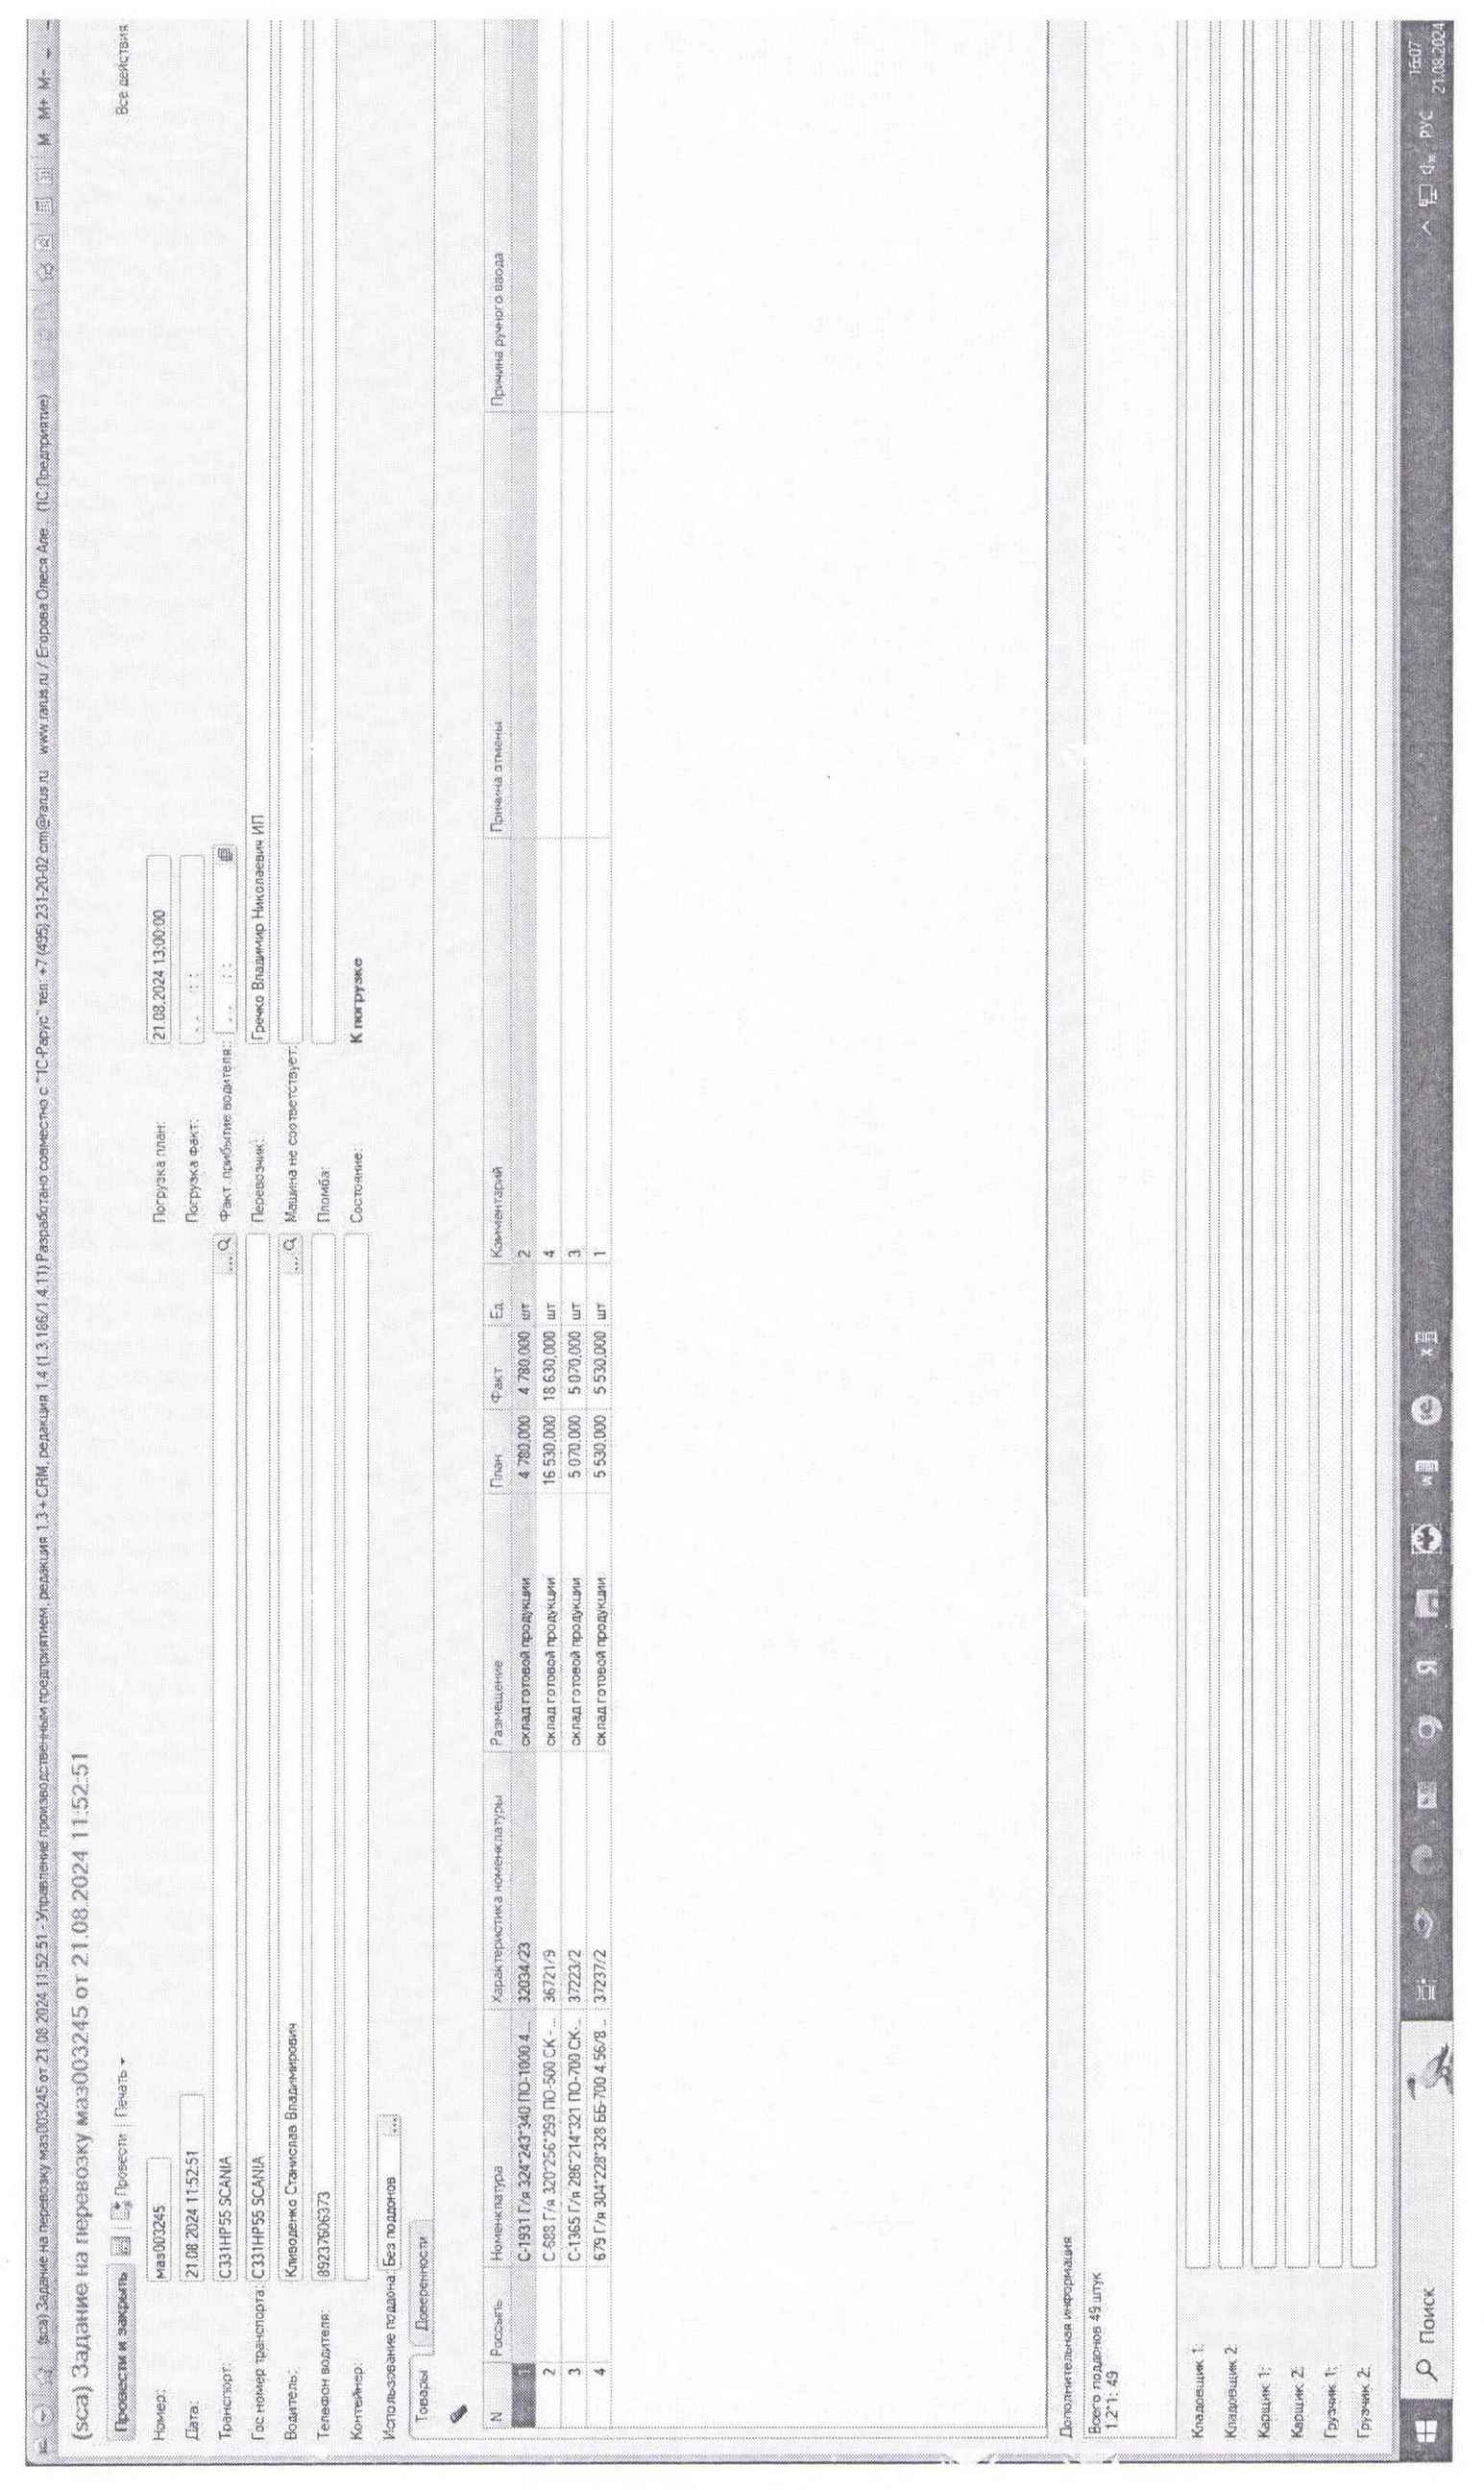
\includegraphics[height=0.8\textheight, width=0.8\textwidth, keepaspectratio]{Pics/d25.jpg}
\end{center}
  \caption{Задание на отгрузку в системе 1С:УПП}
  \label{pic:d25}
\end{figure}



\begin{figure}
\begin{center}
  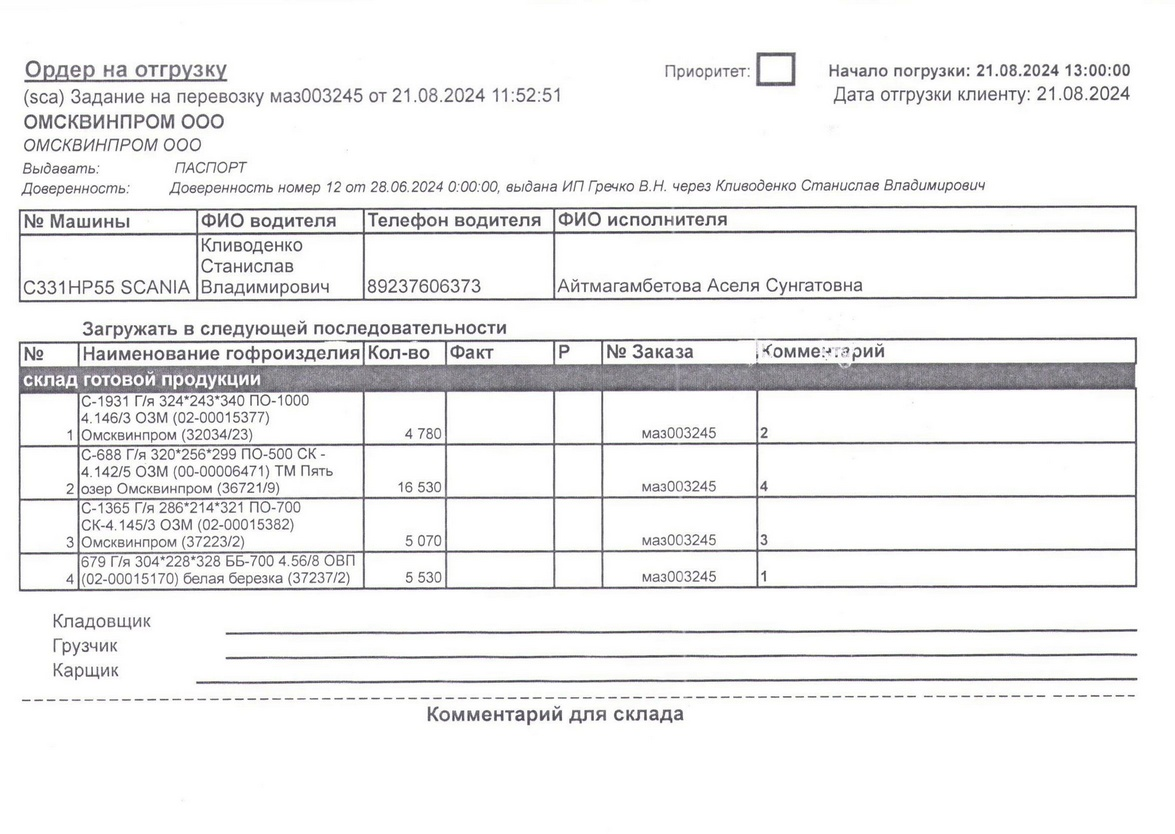
\includegraphics[height=0.6\textheight, angle=90, keepaspectratio]{Pics/d27.jpg}
\end{center}
  \caption{Печатная форма ордера на отгрузку}
  \label{pic:d27}
\end{figure}

\begin{figure}
\begin{center}
  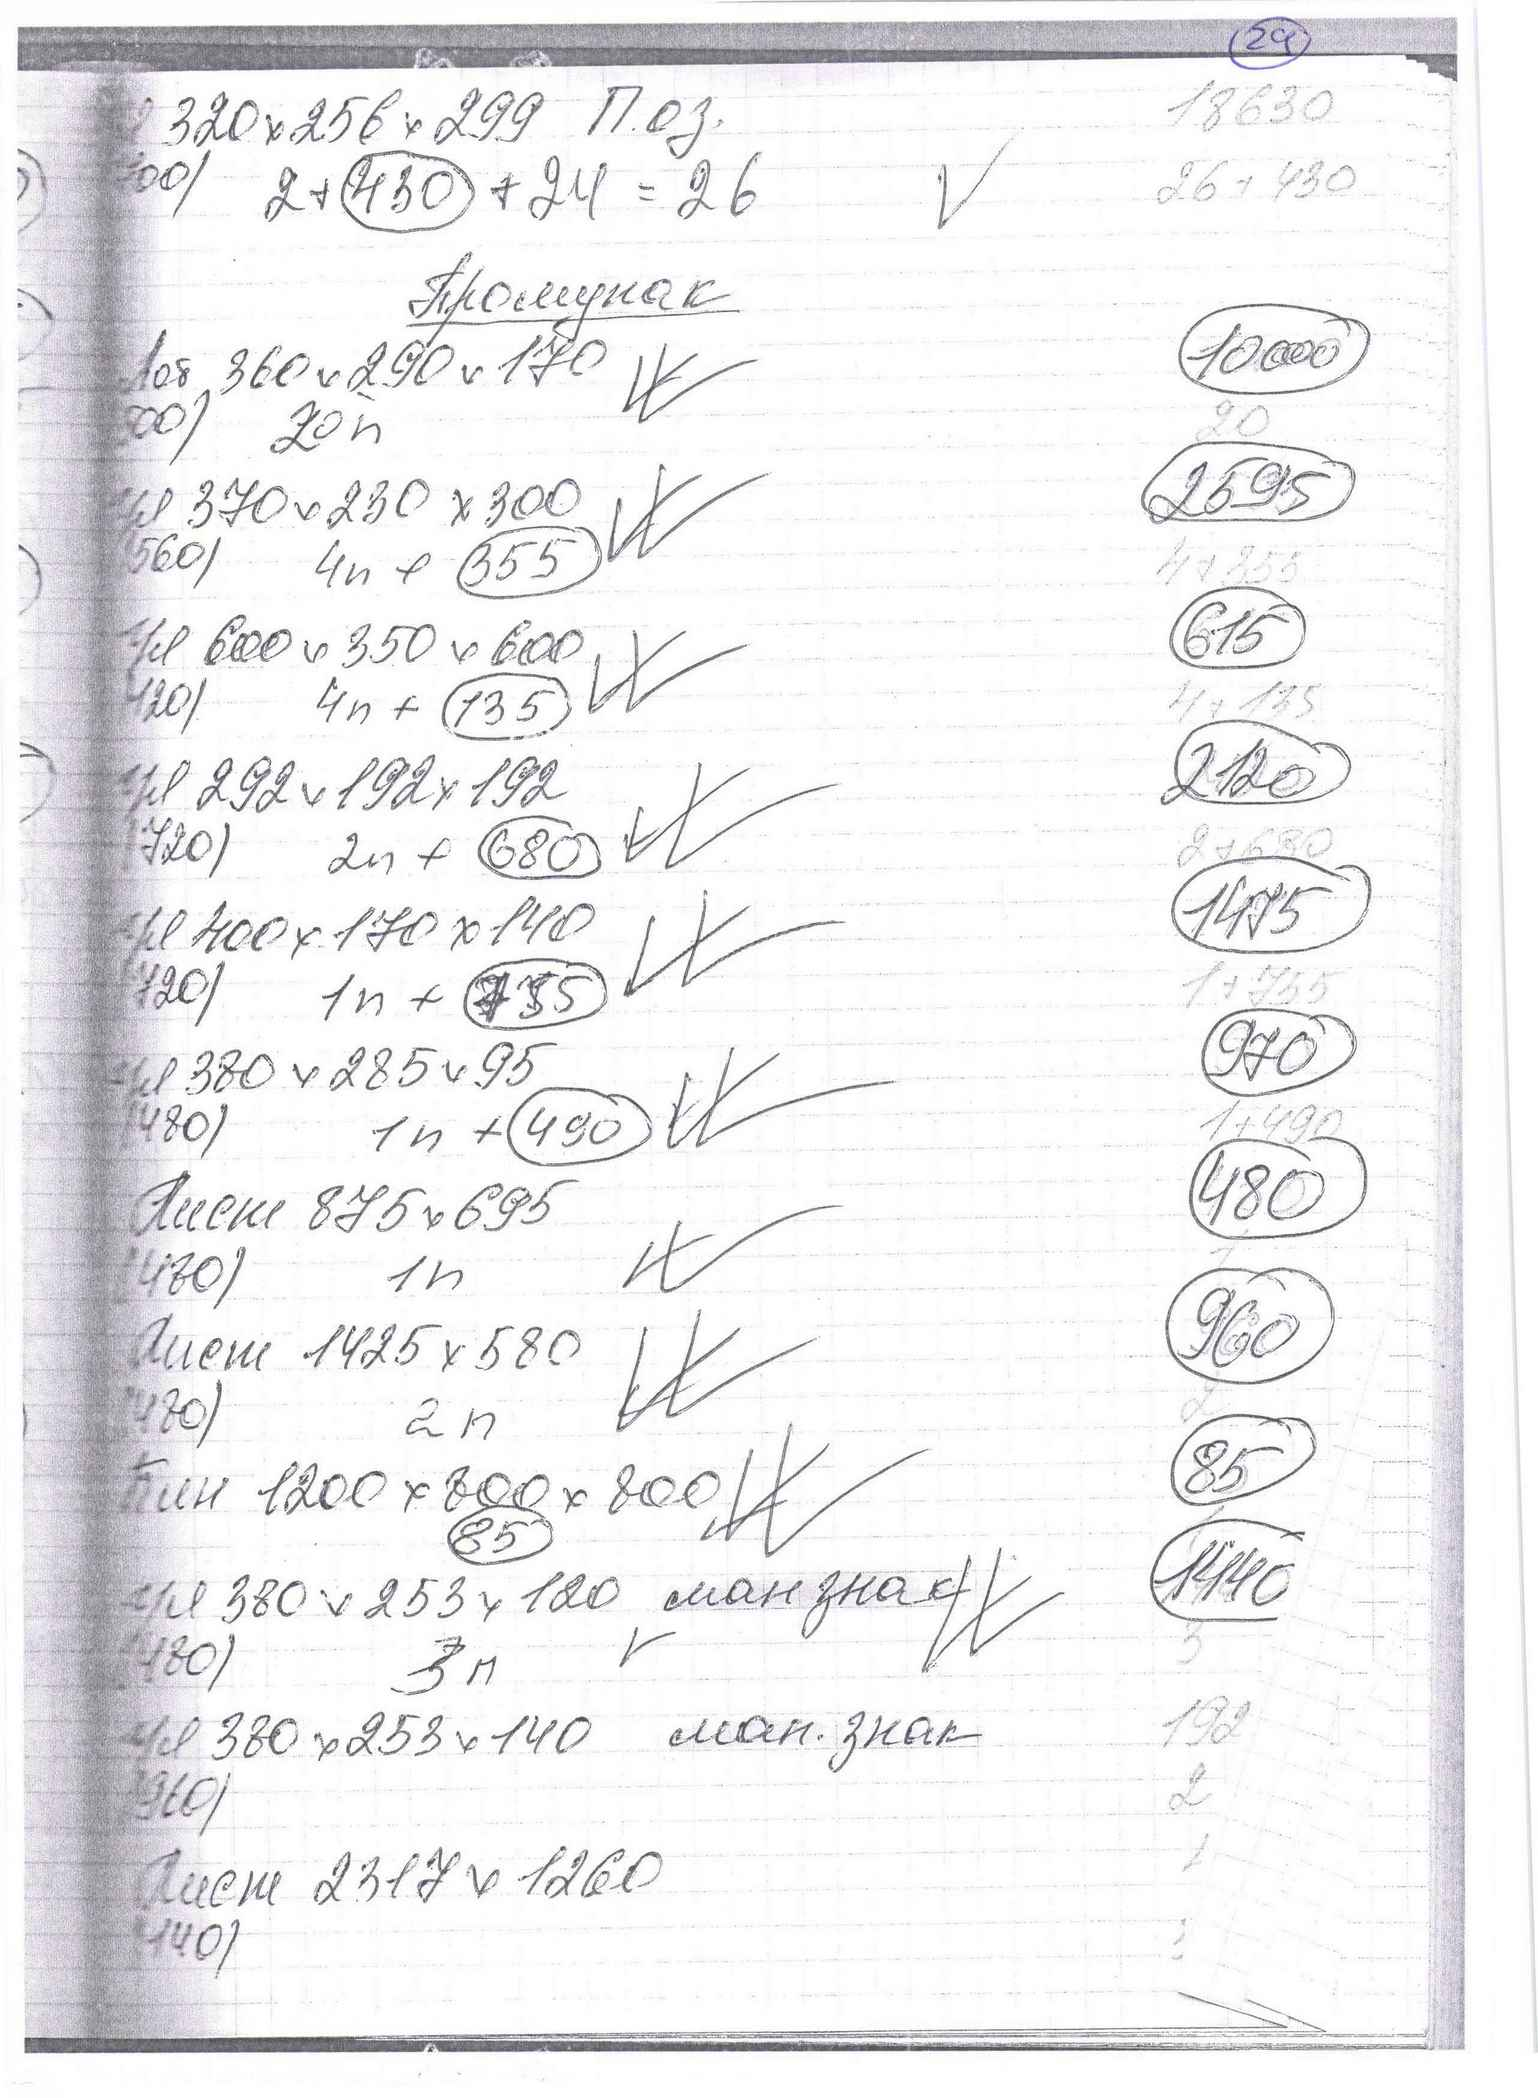
\includegraphics[height=0.8\textheight, keepaspectratio]{Pics/d28.jpg}
\end{center}
  \caption{Журнал остатков по готовой продукции}
  \label{pic:d28}
\end{figure}


\begin{figure}
\begin{center}
  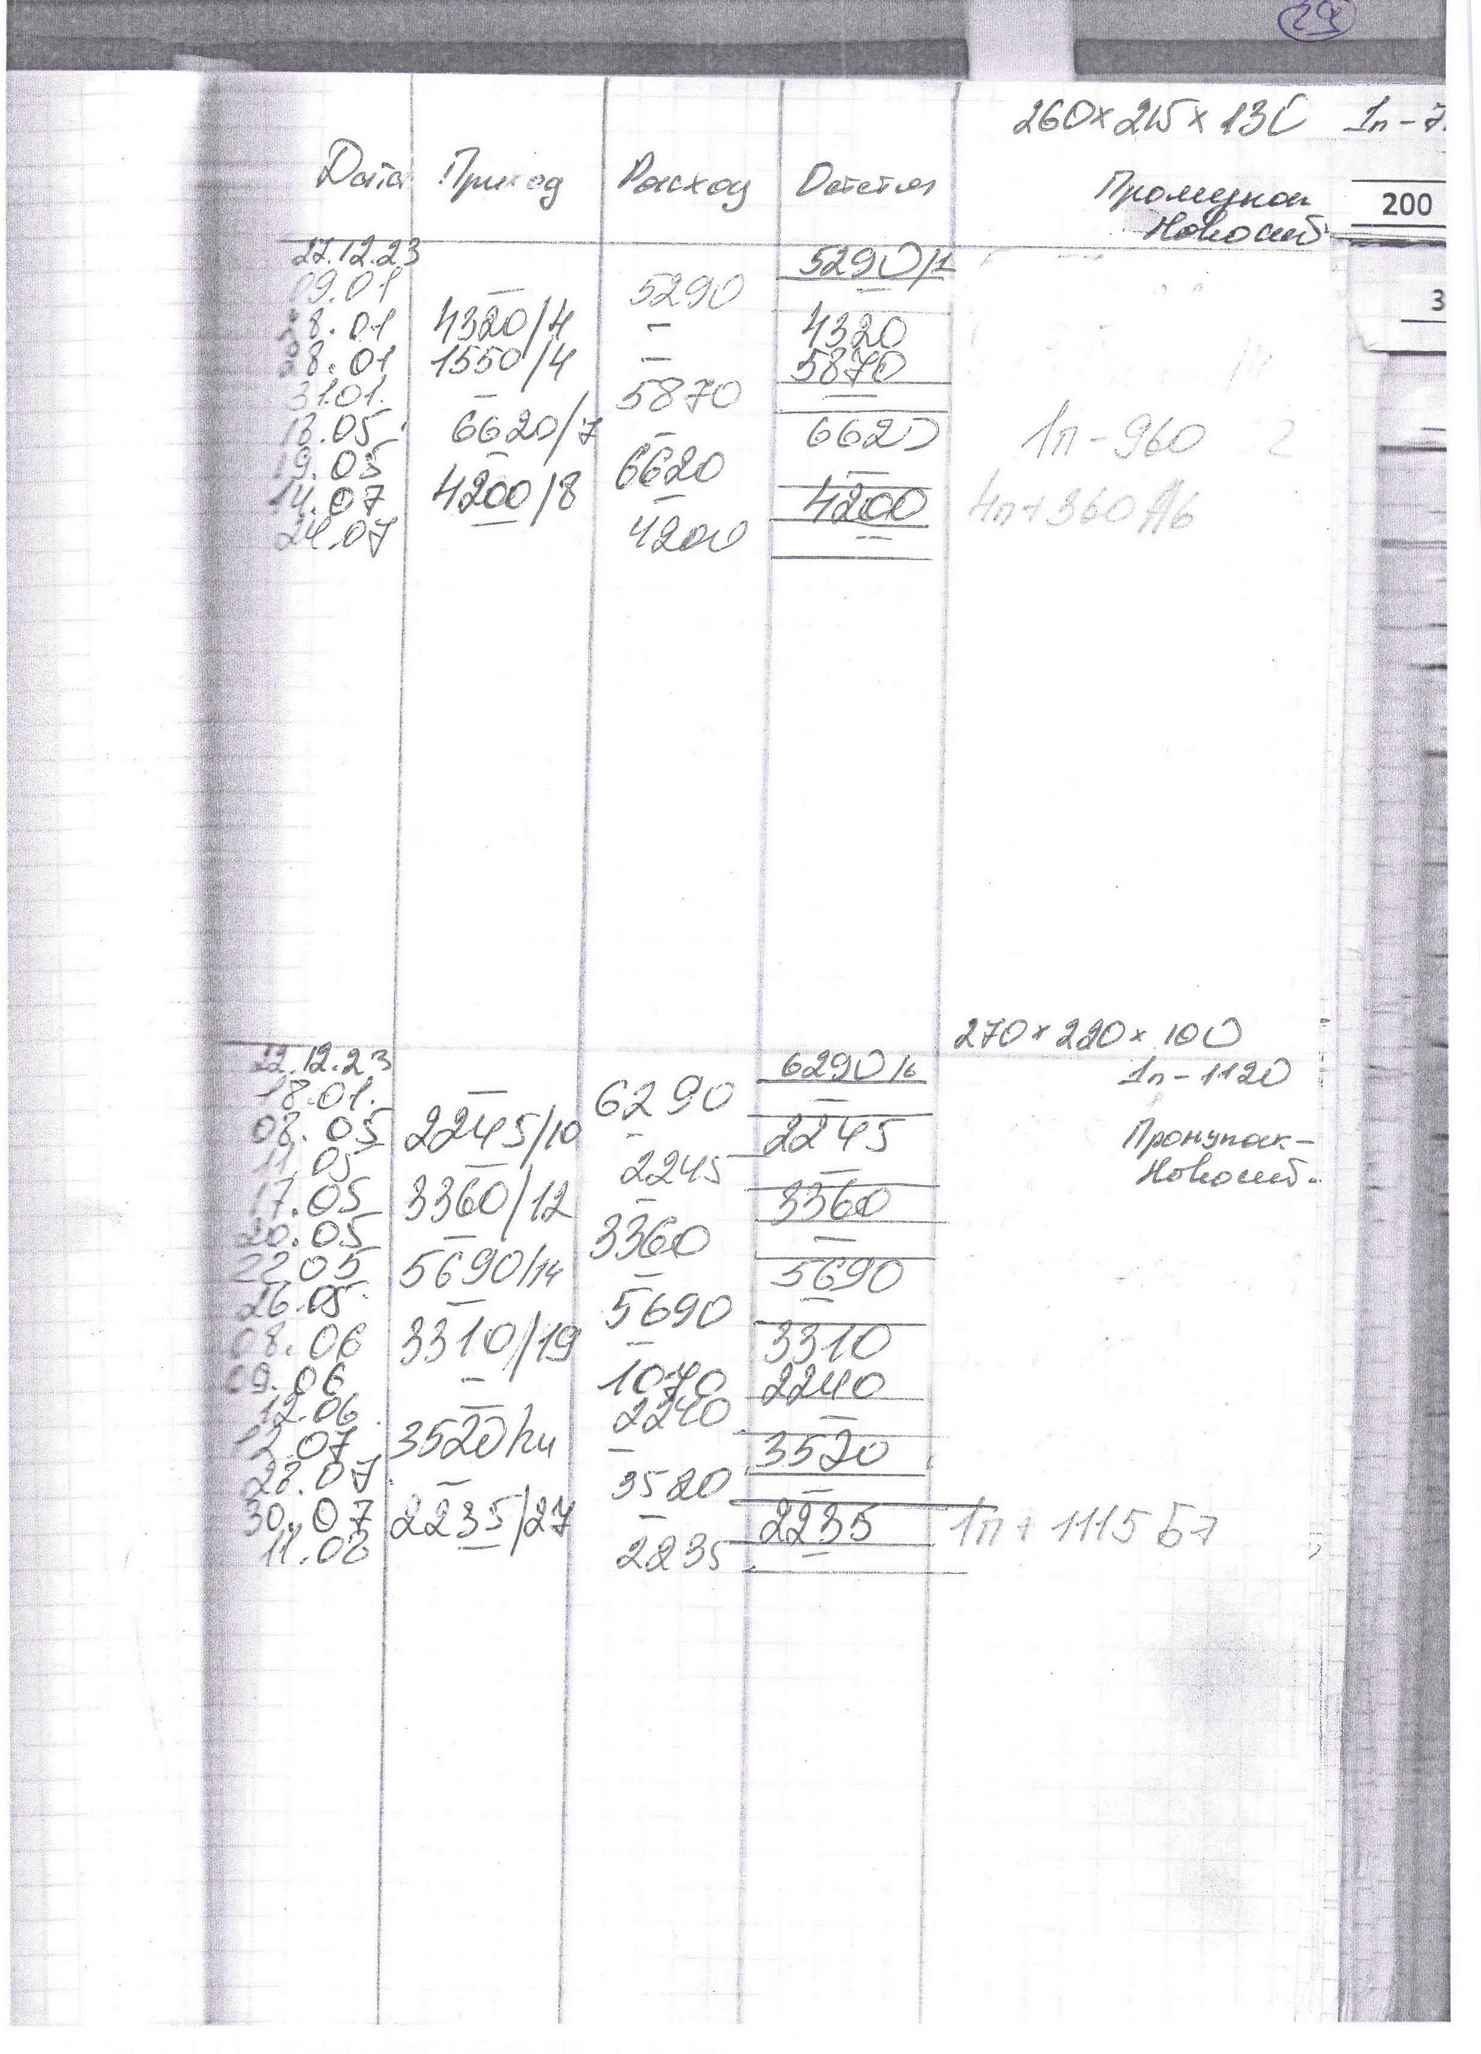
\includegraphics[height=0.8\textheight, keepaspectratio]{Pics/d29_2.jpg}
\end{center}
  \caption{Журнал отгрузки по готовой продукции}
  \label{pic:d29}
\end{figure}

\begin{figure}
\begin{center}
  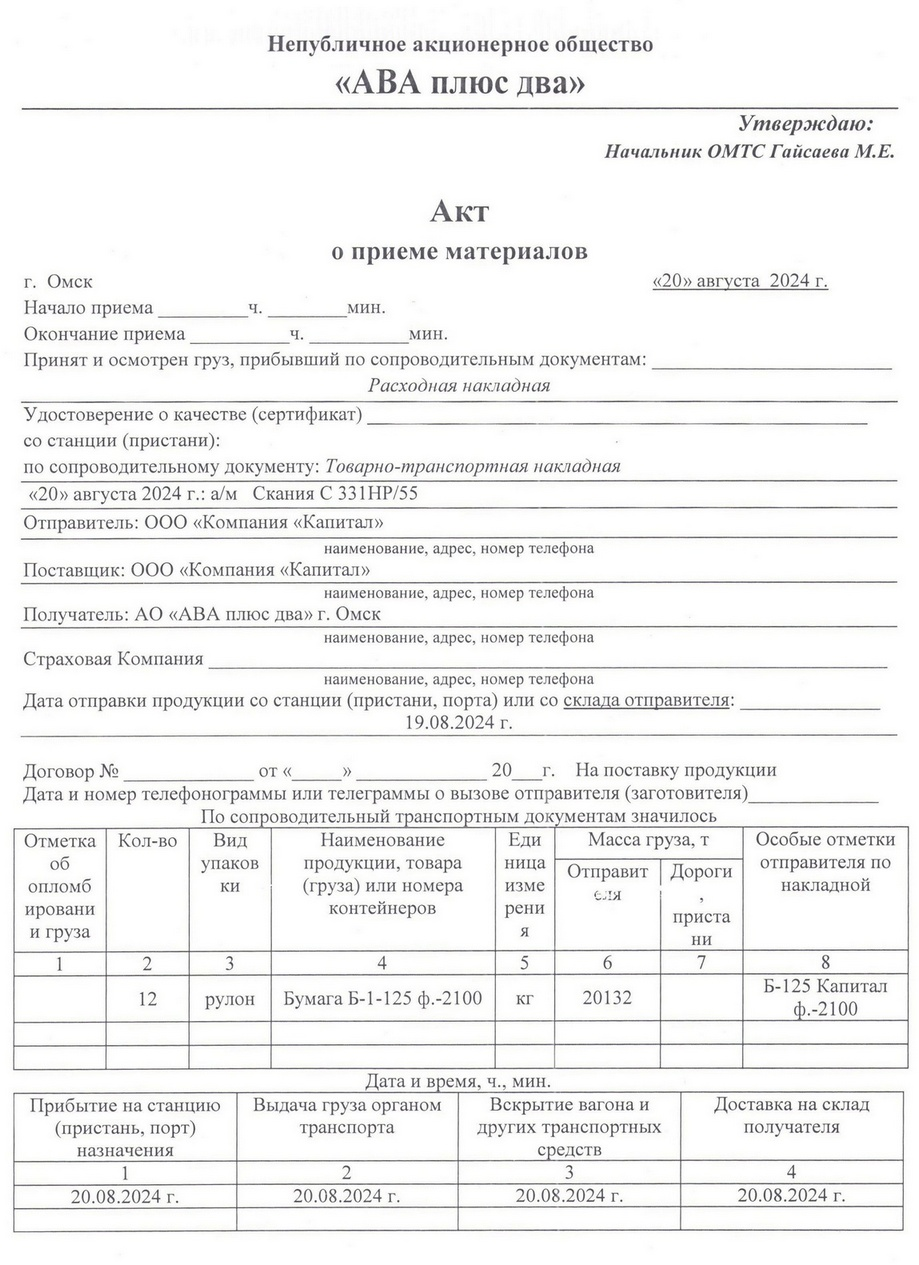
\includegraphics[height=0.8\textheight, keepaspectratio]{Pics/d33.jpg}
\end{center}
  \caption{Акт по приемке материалов}
  \label{pic:d33}
\end{figure}




% Графика подачи машин не выявлено. Машины на погрузку подъезжают в порядке очереди.
% По факту поступления машины кладовщик принимает машину. 
% Кладовщик грузит готовую продукцию по факту на основании плана погрузки и заявки из 1С. Остатки могут остаться на складе. 
% Кладовщик отмечает в заявке покупателя факт отгрузки, передает в отдел учета.

% Кладовщик по отгрузке или мастер смены ночью пишет накладную (рис. \ref{pic:d17}).
% Машина ночью грузится, но ее не отпускают.
% Кладовщик на площадке 1 пишет накладную (рис. \ref{pic:d18}), сканирует и высылает в отдел складской логистики. 
%  По второй площадке Кладовщики пишут заявку покупателя. 
% % (рис. \ref{pic:d19}).
% Кладовщик сам печатает другие бирки на складе по готовой продукции, меняет дату, клиента (рис. \ref{pic:d40}).

% В Google Tab Кладовщики меняет списание по факту.
% Существуют заявки от менеджеров, где указывается количество листов по готовой продукции (рис. \ref{pic:d41}).
% Менеджер может попросить отгрузить другое количество, чем указано в упаковке на паллете (рис. \ref{pic:d42}). Кладовщик может разукомплектовать чужой паллет при необходимости. При этом перепечатывает бирку.

 
% Кладовщик пишет накладную (рис. \ref{pic:d43}), сканирует, отправляет оператору по емайл. Оператор 1С создает в системе 1С: Бухгалтерия накладную, печатает сопроводительные документы, передает водителю.


% Отдел складской логистики на основании накладных (рис. \ref{pic:d17}, \ref{pic:d18})
% % или \ref{pic:d19}) 
% выписывает расходную накладную в системе 1С: Бухгалтерия (упр) и в реальной 1С: Бухгалтерия по юридическому лицу, указанному в заявке.
% В заявке на поставку указано юридическое лицо, от которого будет реализация.
% Отдел логистики печатает расходную накладную и при необходимости пакет сопроводительных документов.

% Паспорта качества по готовой продукции не печатаются.

% В течение дня 
% % по форме \ref{pic:d19}
% оператор 1С создает документ ''Отчет производства за смену''. На основании документа ''Реализация'' учетчик создает в системе 1С Бухгалтерия документ ''Перемещение'' с производства на склад и документ ''Реализация'' по факту отгрузки.

% По площадке 1 учетчик получает заявку на отгрузку. В системе 1С Бухгалтерия создает документ ''Поступление ТМЦ'', ''Перемещение'' и ''Реализация''. Форму накладной отсылает почтой на склад.
% Учетчик регистрирует поступление готовой продукции только в системе 1С Бухгалтерия (Упр). В информационной базе 1С по 
% ИМ Макаров учетчик создает только документ ''Реализация''. В информационной базе 1С по фирме  Норд-Пак учетчик создает документ ''Отчет производства за смену'' и документ ''Реализация''.




% \begin{figure}
% \begin{center}
%   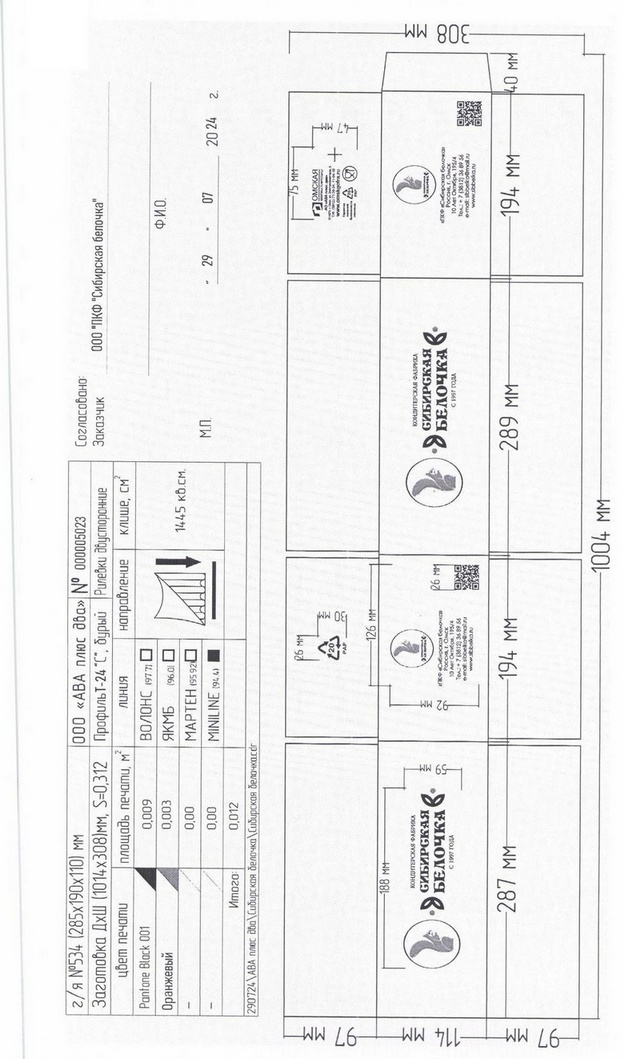
\includegraphics[height=0.94\textheight, keepaspectratio]{Pics/d17.jpg}
% \end{center}
%   \caption{Накладная на отгрузку готовой продукции площадка 3}
%   \label{pic:d17}
% \end{figure}

% \begin{figure}
% \begin{center}
%   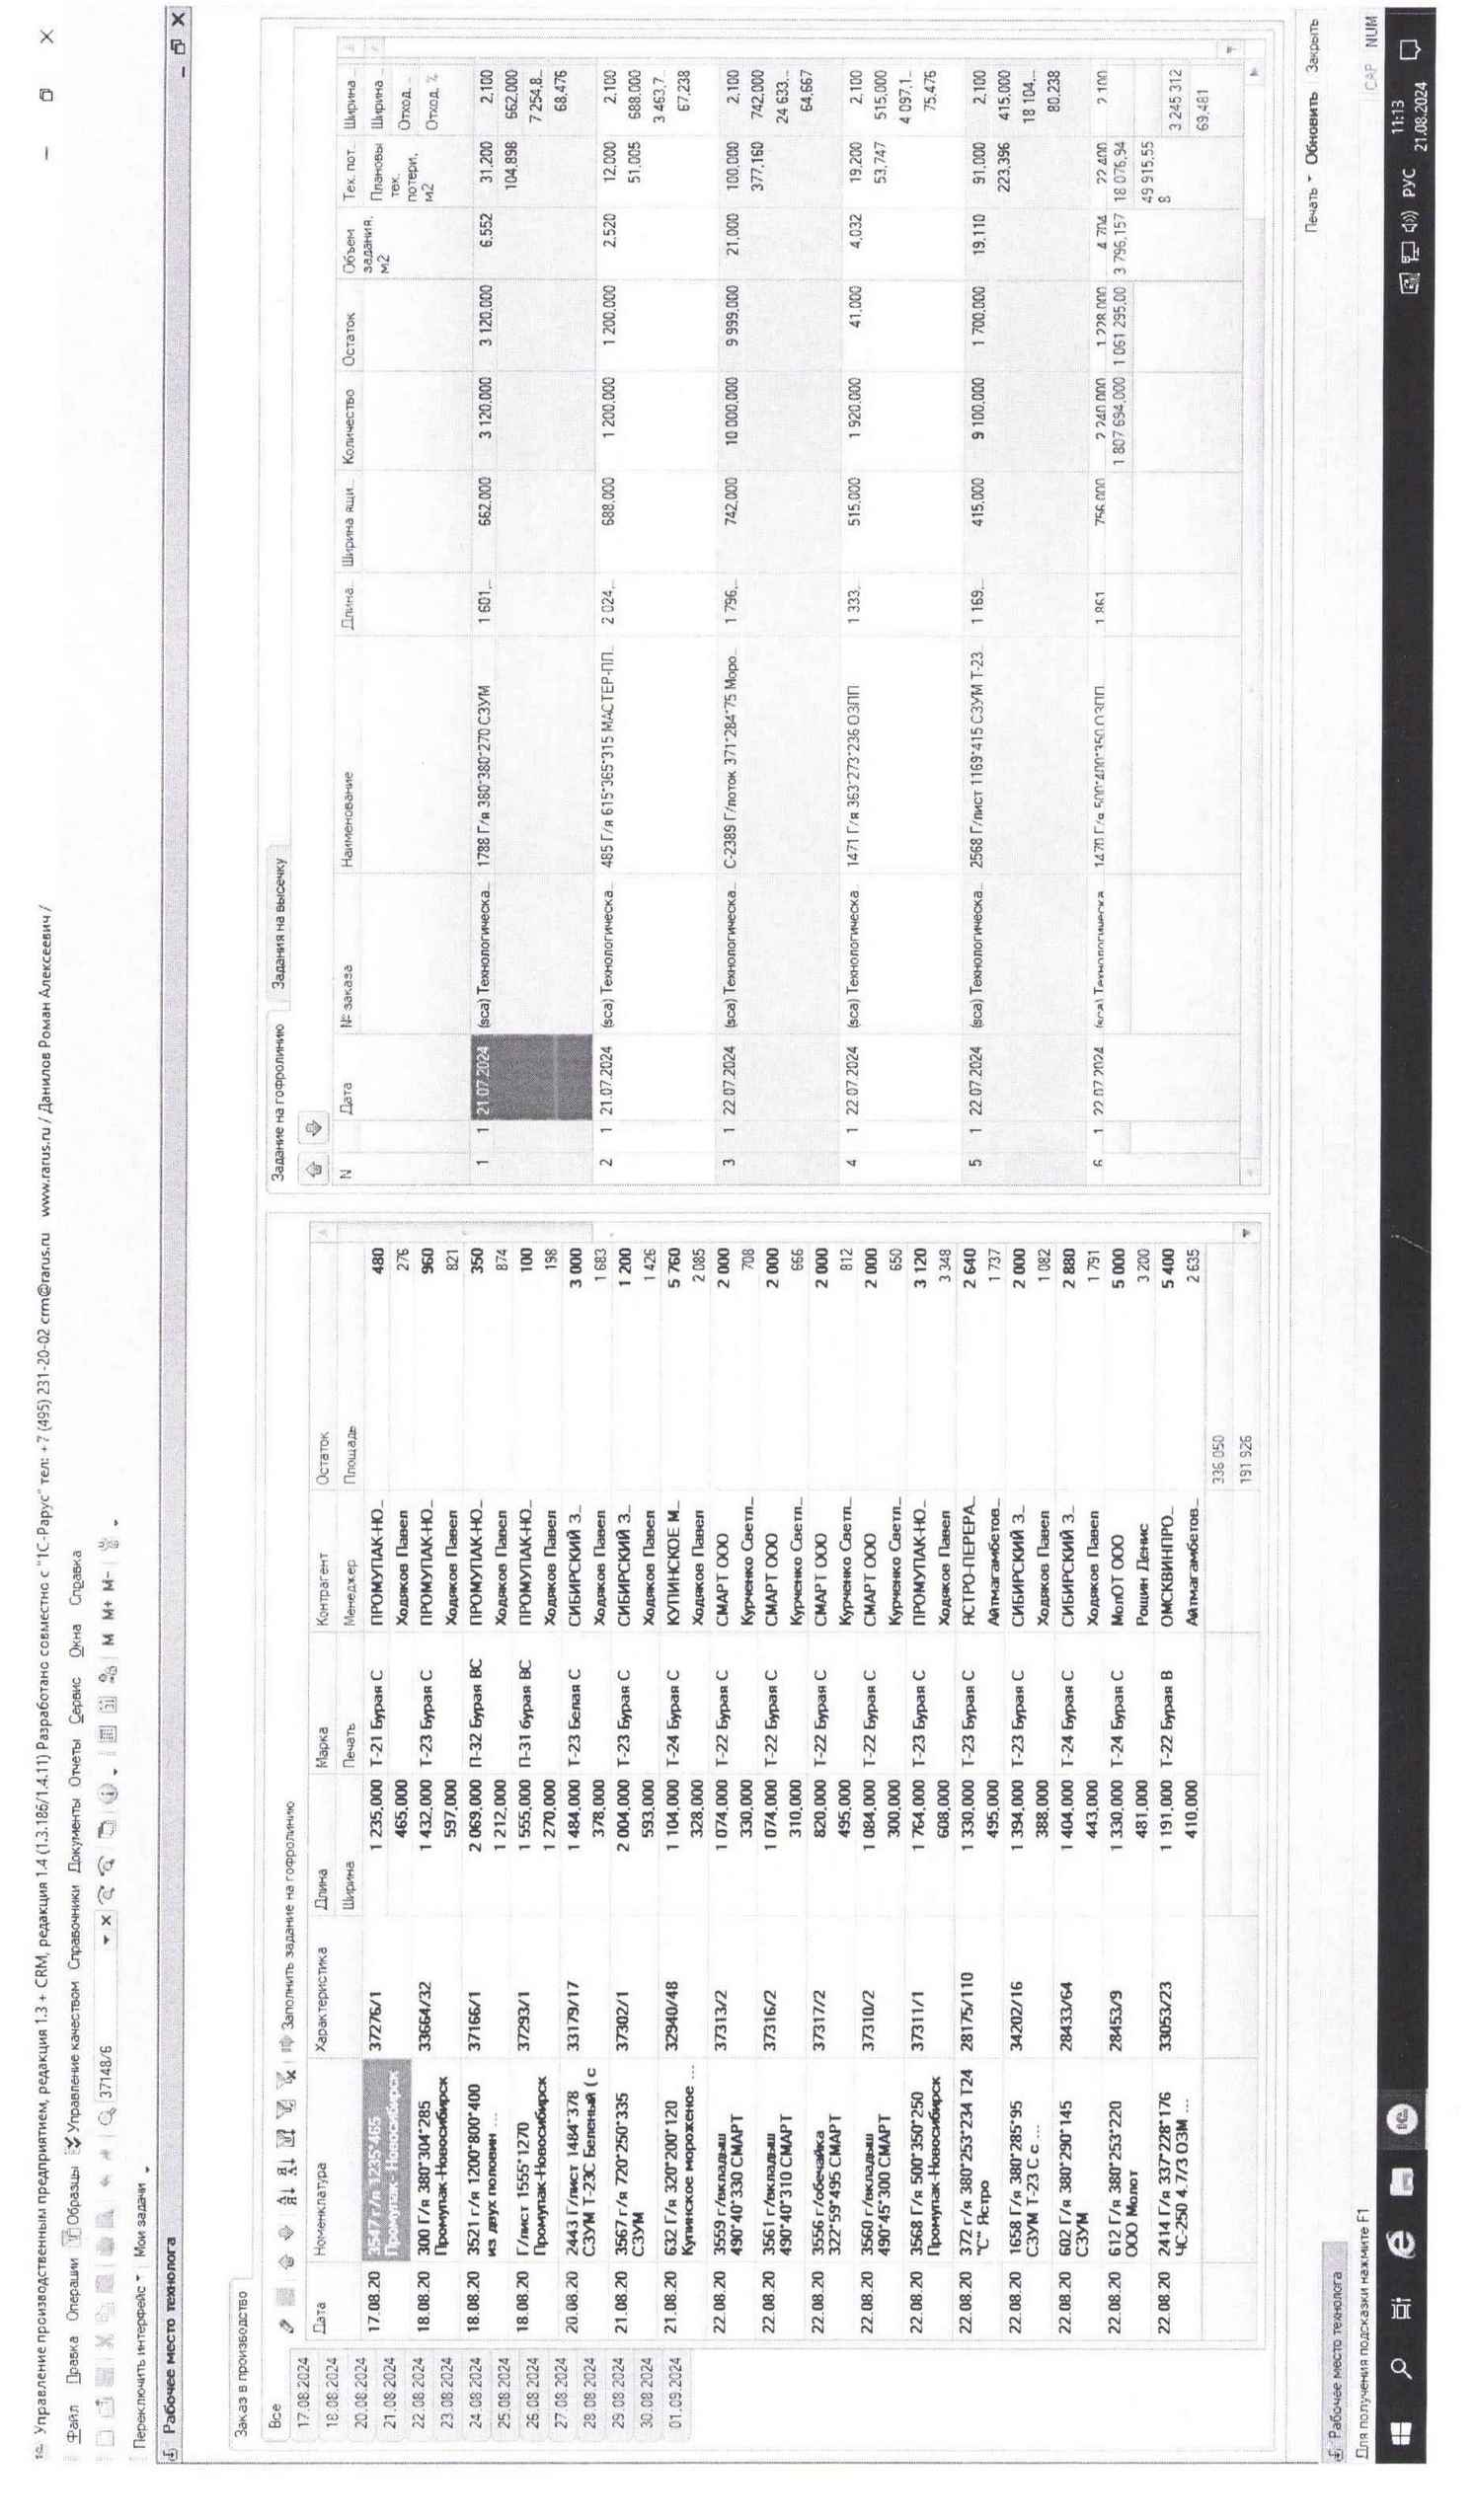
\includegraphics[height=0.94\textheight, keepaspectratio]{Pics/d18.jpg}
% \end{center}
%   \caption{Накладная на отгрузку готовой продукции площадка 1}
%   \label{pic:d18}
% \end{figure}




% \begin{figure}
% \begin{center}
%   \includegraphics[height=0.94\textheight, keepaspectratio]{Pics/d43.jpg}
% \end{center}
%   \caption{Накладная на отгрузку готовой продукции площадка 2}
%   \label{pic:d43}
% \end{figure}

\clearpage